\documentclass[tikz,border=8pt]{standalone}
\usepackage[scaled=0.95]{helvet}
\renewcommand{\familydefault}{\sfdefault}
\usetikzlibrary{arrows.meta,decorations.pathmorphing}
\definecolor{TEJNavy}{HTML}{1E2B55}
\definecolor{TEJBlue}{HTML}{1769AA}
\definecolor{TEJRed}{HTML}{B3261E}
\begin{document}
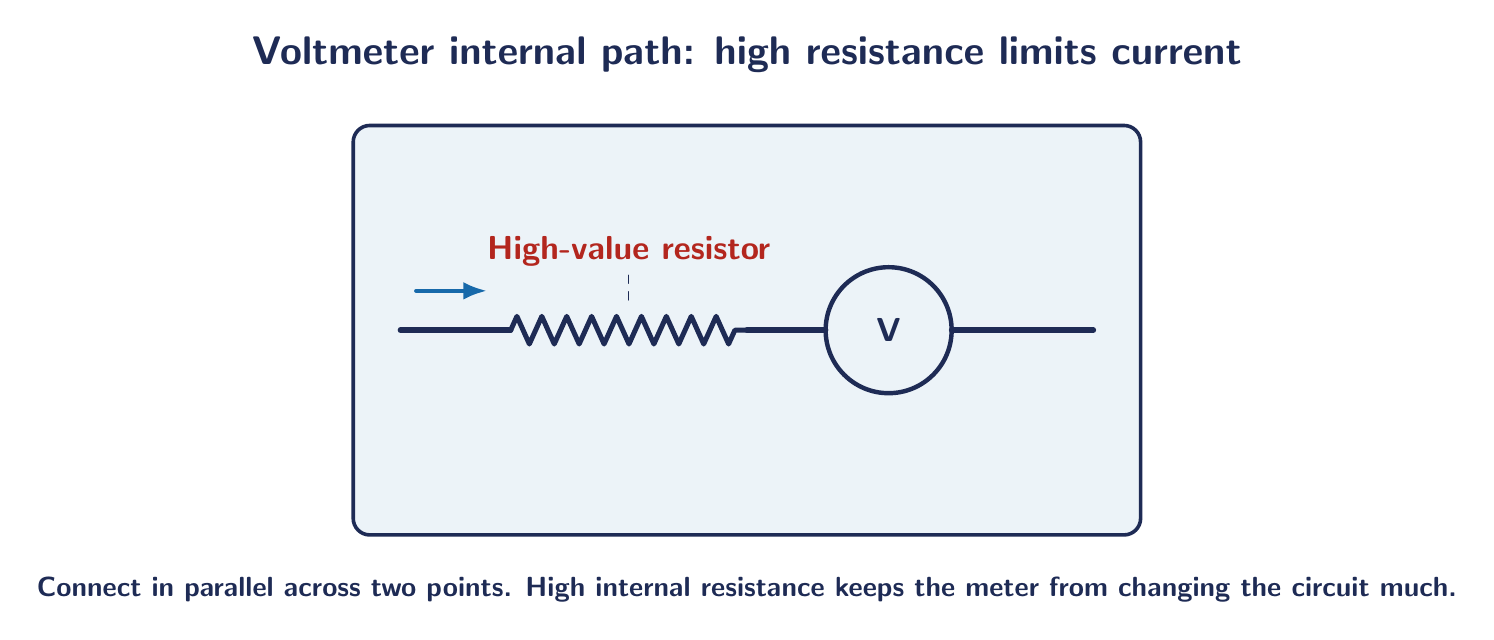
\begin{tikzpicture}[line cap=round,line join=round,font=\sffamily]
  \filldraw[fill=TEJBlue!8,draw=TEJNavy,line width=1.3pt,rounded corners=6pt] (0,0) rectangle (10,5.2);
  \draw[TEJNavy,line width=2pt] (0.6,2.6) -- (2.0,2.6);
  \draw[TEJNavy,line width=1.8pt,decorate,decoration={zigzag,segment length=9pt,amplitude=5pt}] (2.0,2.6) -- (5.0,2.6);
  \draw[TEJNavy,line width=2pt] (5.0,2.6) -- (6.0,2.6);
  \draw[TEJNavy,line width=1.6pt] (6.8,2.6) circle (0.8);
  \draw[TEJNavy,line width=2pt] (7.6,2.6) -- (9.4,2.6);
  \node[font=\bfseries\Large,text=TEJNavy] at (5,6.1) {Voltmeter internal path: high resistance limits current};
  \node[font=\bfseries\large,text=TEJRed] at (3.5,3.6) {High-value resistor};
  \draw[TEJNavy,dashed] (3.5,3.3) -- (3.5,2.9);
  \node[font=\bfseries\large,text=TEJNavy] at (6.8,2.6) {V};
  \draw[-{Latex[length=3mm]},TEJBlue,line width=1.5pt] (0.8,3.1) -- (1.7,3.1);
  \node[font=\bfseries,text=TEJNavy,align=center] at (5,-0.7) {Connect in parallel across two points. High internal resistance keeps the meter from changing the circuit much.};
\end{tikzpicture}
\end{document}
